%%%%%%%%%%%%%%%%%%%%%%%%%%%%%%%%%%%%%%%%%%%%%%%%%%%%%%%%%%%%
%% filename:	vortrag.tex
%% template:	Mon, 07 May 2012 13:01:14 +0200
%% author:	Hermann Lorenz
%% date:	20. Nov 2012 10:00
%%%%%%%%%%%%%%%%%%%%%%%%%%%%%%%%%%%%%%%%%%%%%%%%%%%%%%%%%%%%
\documentclass[%
	ngerman%
	]{beamer}

%\setbeameroption{show only notes} 	% note{} -- Anmerkungsfolien


%%%%%%%%%%%%%%%%%%%%%%%%%%%%%%%%%%%%%%%%%%%%%%%%%%%%%%%%%%%%
%% Lokalisierung %%%%%%%%%%%%%%%%%%%%%%%%%%%%%%%%%%%%%%%%%%%
%%%%%%%%%%%%%%%%%%%%%%%%%%%%%%%%%%%%%%%%%%%%%%%%%%%%%%%%%%%%
\usepackage[utf8]{inputenc}	% Umlaute direkt eingeben
\usepackage[T1]{fontenc}	% Wörter mit Umlaute umbrechen
\usepackage[ngerman]{babel}	% deutsche Bezeichner
\usepackage[babel,german=guillemets]{csquotes}	% \enquote{}
\usepackage{libertine}
\usepackage[scaled=0.83]{beramono}


%%%%%%%%%%%%%%%%%%%%%%%%%%%%%%%%%%%%%%%%%%%%%%%%%%%%%%%%%%%%
%% Bilder %%%%%%%%%%%%%%%%%%%%%%%%%%%%%%%%%%%%%%%%%%%%%%%%%%
%%%%%%%%%%%%%%%%%%%%%%%%%%%%%%%%%%%%%%%%%%%%%%%%%%%%%%%%%%%%
\usepackage{graphicx}	% \includegraphics{bild.pdf}
\usepackage{tikz}

%-----------------------------------------------------------
% TikZ library: arrows, positioning

\usetikzlibrary{arrows,positioning}
\tikzset{
    %Define standard arrow tip
    >=stealth',
    %Define style for boxes
    punkt/.style={
           rectangle,
           rounded corners,
           draw=black, very thick,
           text width=6.5em,
           minimum height=2em,
           text centered},
    % Define arrow style
    pil/.style={
           ->,
           thick,
           shorten <=2pt,
           shorten >=2pt,}
}
\usetikzlibrary{fit}

%%%%%%%%%%%%%%%%%%%%%%%%%%%%%%%%%%%%%%%%%%%%%%%%%%%%%%%%%%%%
%% pdf-links %%%%%%%%%%%%%%%%%%%%%%%%%%%%%%%%%%%%%%%%%%%%%%%
%%%%%%%%%%%%%%%%%%%%%%%%%%%%%%%%%%%%%%%%%%%%%%%%%%%%%%%%%%%%
\usepackage[ngerman]{varioref}	% \vpageref{}

%%%%%%%%%%%%%%%%%%%%%%%%%%%%%%%%%%%%%%%%%%%%%%%%%%%%%%%%%%%%
%% eigene Macros %%%%%%%%%%%%%%%%%%%%%%%%%%%%%%%%%%%%%%%%%%%
%%%%%%%%%%%%%%%%%%%%%%%%%%%%%%%%%%%%%%%%%%%%%%%%%%%%%%%%%%%%
\usepackage{xspace}

\newcommand{\zB}{z.\,B.\xspace}
\newcommand{\conclusion}{\(\to\)\xspace}

\newcommand{\todo}[1]{\textcolor{red}{TODO: #1}}
\newcommand{\prove}[1]{\textcolor{red}{TODO/PROVE(#1)}}
%\newcommand{\todo}[1]{}
%\newcommand{\prove}[1]{}

\definecolor{lgray}{gray}{.3}
\newcommand{\notall}[1]{\textcolor{lgray}{#1}}
\newcommand{\eg}[1]{\textcolor{lgray}{#1}}

\newcommand{\noteparagraph}[1]{\smallskip \textbf{#1}\,\,}

\setbeamertemplate{frametitle}{
	\hspace{-1.5em}
	\insertframetitle\\
	\hspace{-.5em}\scriptsize\insertframesubtitle\hfill\insertpart\\[-.9em]
	\rule{\textwidth}{.1pt}
}
\setbeamertemplate{frametitle}{%
	\renewcommand{\arraystretch}{0.5}
	\begin{tabular}{@{}l}
		\hspace{-1.5em}
		\insertframetitle \tabularnewline
		\hspace{-.5em}
		\scriptsize\insertframesubtitle \tabularnewline
	\end{tabular}
	\hfill%
	{\scriptsize\insertpart}\\[-.5em]
	\rule{\textwidth}{.1pt}
}
\setbeamertemplate{footline}{
	\usebeamercolor[fg]{structure}
	\hspace*{.5cm}\raisebox{3pt}{
	\begin{tikzpicture}
		\draw [draw opacity=0.0] (-2pt,0) -- (.85\textwidth + 2pt,0) -- (.85\textwidth + 2pt,-5pt) -- (-2pt,-5pt) -- cycle;
		\draw (0,0) -- (.85\textwidth,0);
		\ifnum\inserttotalframenumber>1
		\if \insertpartstartpage \insertpartendpage
		\else
		\draw [fill,xshift=.85\textwidth / (\insertpartendpage - \insertpartstartpage) * (\insertpagenumber - \insertpartstartpage)] (0,0) -- (2pt,-5pt) -- (-2pt,-5pt) -- cycle;
		\fi
		\fi
	\end{tikzpicture}
	}
	\hfill\raisebox{3pt}{\insertframenumber/\inserttotalframenumber\hspace{3pt}}
}

\definecolor{hllgreen}{rgb}{.2,.7,.2}
\definecolor{hllgreenbg}{rgb}{.9,1,.9}
\definecolor{hllblue}{rgb}{.2,.2,.7}
\definecolor{hllbluebg}{rgb}{.9,.9,1}
\definecolor{hllorange}{rgb}{1,0.482,0}
\definecolor{hllorangebg}{rgb}{1,0.782,.4}
\setbeamertemplate{blocks}[rounded]
\setbeamercolor{structure}{fg=hllblue}
\setbeamercolor{normal text}{fg=black}
\setbeamercolor{alerted text}{fg=hllorange}
\setbeamercolor{block title alerted}{fg=black,bg=hllorange}
\setbeamercolor{block body alerted}{fg=black,bg=hllorangebg}
\setbeamercolor{block title}{fg=white,bg=hllblue}
\setbeamercolor{block body example}{fg=black,bg=hllgreenbg}
\setbeamercolor{block title example}{fg=white,bg=hllgreen}
\setbeamercolor{block body}{fg=black,bg=hllbluebg}

\newcommand{\prosymbol}{%
	\raisebox{-.1\baselineskip}{%
		\begin{tikzpicture}%
			\draw [line width=.1\baselineskip] (-.25\baselineskip,0) -- (.25\baselineskip,0);%
			\draw [line width=.1\baselineskip] (0,-.25\baselineskip) -- (0,.25\baselineskip);%
		\end{tikzpicture}%
	}%
	}
\newcommand{\contrasymbol}{%
	\raisebox{.15\baselineskip}{%
		\begin{tikzpicture}%
			\draw [line width=.1\baselineskip] (-.25\baselineskip,0) -- (.25\baselineskip,0);%
		\end{tikzpicture}%
	}%
	}
\definecolor{procolor}{rgb}{0,.8,0}
\definecolor{contracolor}{rgb}{.8,0,0}
%         |
%         |
%         |
%   ------+------
%         |
%         |
%         |
%
% h = .5\baselineskip
%
%
%   -------------
% h = .1\baselineskip
%
%
\newenvironment{proconlist}%
	{%
		\begin{list}{?}{}%
		\newcommand{\pro}{\item[\textcolor{procolor}{\prosymbol}]}%
		\newcommand{\contra}{\item[\textcolor{contracolor}{\contrasymbol}]}%
	}{%
		\end{list}%
	}


\usepackage{listings}
\lstset{basicstyle=\ttfamily\scriptsize,backgroundcolor=\color[rgb]{.9,.9,.9}}
\usepackage{dirtree}

\usepackage{tabularx}
\usepackage{multirow}
\usepackage{booktabs}
\usepackage{bbding}
\usepackage[squaren]{SIunits}

\AtBeginSection{%
	\begin{frame}{Übersicht}%
		\tableofcontents[currentsection]%
	\end{frame}%
}

%-------------------------------------------------------------------------------
% Navigationsleiste ausblenden
\setbeamertemplate{navigation symbols}{}

%-------------------------------------------------------------------------------
% Diesen Abschnitt über \begin{document} lassen, damit die PDF-Informationen
% korrekt gesetzt werden.
\title{Forschungsprojekt Sensornetze}
\date{10.\,Dezember~2012}
\author{Angelos~Drossos \and Hermann~Lorenz
	\and Ulrich~Meckel \and Martin~Doenicke
	\and Thomas~Bettermann \and Robert~Krampe 
	\and Marcus~Kupke \and Markus~Fischer
	\and Enrico~Uhlig}
\institute{Hochschule für Technik und Wirtschaft Dresden\\%
			Master Angewandte Informationstechnologien\\%
			Forschungsprojekt Sensornetze\\%
			Prof. Dr. J. Vogt%
}
%-------------------------------------------------------------------------------

\begin{document}
%-------------------------------------------------------------------------------
\begin{frame}[plain]
	\maketitle
\end{frame}

%-------------------------------------------------------------------------------
\section{Einführung}
\myContentSectionFrame

%----------------------------------------------------------

\subsection{Gebäude- vs. Hausautomatisierung}

%----------------------------------------------------------

\begin{frame}{Abgrenzung von Haus- und Gebäudeautomatisierung}{Gebäudeautomatisierung}
	\begin{itemize}
	\item 	wichtiger Bestandteil des technischen Facility-Managements
	\item 	Energie- und Personaleinsparungen stehen im Vordergrund
	\item 	dezentrale Anordnung der Steuerungseinheiten
	\item 	Funktionsabläufe gewerkeübergreifend automatisch durchführen
	\item 	Visualisierung der Automation nebensächlich\newline
			(nur in der Managementebene)
	\item 	i.\,d.\,R. herstellerspezifische, kommerzielle Bussysteme
	\item 	Trend zur Offenheit und zum herstellerübergreifenden Informationsaustausch
			(\emph{Interoperabilität}\,)
			% Lockerung der Herstellerabhängigkeit (kein OpenSource-Gedanke!)
			% Bussystem gibt die Möglichkeit, Fabrikate mehrerer Hersteller
			% ohne größere Probleme miteinander kommunizieren zu lassen.
			% Hersteller generieren für ihre Gateways je nach Projekt
			% politische Preise, um der Interoperabilität entgegen zu wirken.
	\end{itemize}
\end{frame}

%----------------------------------------------------------

\begin{frame}{Abgrenzung von Haus- und Gebäudeautomatisierung}{Hausautomatisierung}
	\begin{itemize}
	\item 	Teilbereich der Gebäudeautomatisierung
	\item 	auf spezielle Bedürfnisse der Bewohner von (privaten) Wohnhäusern zugeschnitten
	\item 	erhöhte Wohnkomfort, Sicherheit der Bewohner und Überwachung im Vordergrund
	\item 	Visualisierung und Interaktion der Bewohner besonders wichtig
	\item 	System muss skalierbar sein
	\item 	neue Geräte müssen leicht installiert werden können
	\end{itemize}
\end{frame}

%----------------------------------------------------------

\subsection{Motivation und Ziel}

\begin{frame}{\insertsubsection}{Vorüberlegungen zur Hausautomatisierung}
	\begin{exampleblock}<+->{bestehende Hausautomatisierungslösungen}
	bestehende Heimautomatisierungen besitzen mindestens einen, meist
	mehrere der folgenden, gravierenden Nachteile:
	\begin{itemize}
	\item	teuer
	\item	proprietär
	\item	schlecht dokumentiert
	\item	wenig Sicherheit (\zB in der Datenübertragung)
	\end{itemize}
	\end{exampleblock}

	% neue Netzwerktechnologien (CoAP, 6LoWPAN, \dots) legen die Möglichkeit
	% nahe, mit ihrer Hilfe eine offene Lösung zu konzipieren

	\begin{block}<+->{Wunsch nach \enquote{freier} Hausautomatisierung}
		\begin{itemize}
		\item 	Hersteller-Unabhängigkeit (Interoperabilität)
		\item 	geringere Installationskosten
		\item 	überschaubarer Wartungsaufwand
		\item 	Regelverarbeitung soll möglichst leicht konfigurierbar sein
		\item 	Stichwort \emph{Internet der Dinge}
		\end{itemize}
	\end{block}
\end{frame}


\section{Heimautomatisierungsserver}

\begin{frame}{Heimautomatisierungsserver}{Systemaufbau}
	\begin{figure}
	\centering
	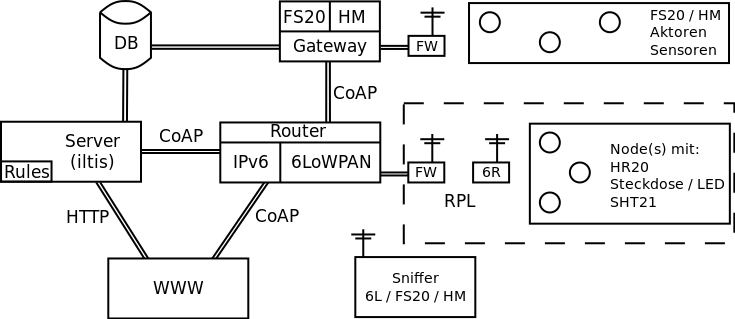
\includegraphics[width=\linewidth]{Systemaufbau}
	%\linebreak
	%\emph{}
	\end{figure}
\end{frame}

\begin{frame}{Heimautomatisierungsserver}{Steuerungsserver und Gateway-Server}
	\begin{block}{Steuerungsserver}
		\begin{itemize}
		\item 	Pairing neuer Geräte
		\item 	Pflegen der angemeldeten Geräte und dessen Sensoren/Aktoren
				(in einer Datenbank)
		\item 	Regelkreis bestimmt Automatisierungsprozess (Regelwerk)
		\end{itemize}
	\end{block}
	\begin{block}{Gateway-Server}
		\begin{itemize}
		\item 	Schnittstelle zwischen CoAP und proprietären Sensornetzen
				\eg(FS20, HomeMatic)
		\item 	Nutzen der Datenbank zur Kategorisierung
		\item 	Caching von Sensorwerten
		\end{itemize}
	\end{block}
\end{frame}

%\subsection{Regelwerk}

%\begin{frame}{Heimautomatisierungsserver}{Regelwerk}
%	\begin{block}{Automatisierung per Regelwerk}
%		\begin{itemize}
%		\item 	\todo{Stand der Technik, vorhandene Lösungen!}
%		\end{itemize}
%	\end{block}

%	\begin{block}{XML als Datenformat}
%		\begin{itemize}
%		\item 	weit verbreitetes Datenformat
%		\item 	Parser in vielen Programmiersprachen vorhanden
%		\item 	XML Schema Validation
%		\item 	in Blockdarstellungen überführbar (für Nutzer)
%		\end{itemize}
%	\end{block}
%\end{frame}

\begin{frame}{Heimautomatisierungsserver}{Anfrage an das Sensornetz}
	\begin{block}{direkte CoAP-Anfragen}
		\begin{itemize}
		\item 	in das 6LoWPAN-Netz ohne Probleme
		\item 	in das FS20/HomeMatic-Netz über Gateway
		\end{itemize}
	\end{block}
	\begin{block}{HTTP-Anfragen auf dem Server}
		\begin{itemize}
		\item 	Mapping von HTTP auf CoAP
		\end{itemize}
	\end{block}
	\begin{block}{Webserver}
		\begin{itemize}
		\item 	Statistiken
		\item 	Erstellung von Regeln
		\item 	Übersicht über alle Sensoren und Aktoren
		\end{itemize}
	\end{block}
\end{frame}


\subsection[REST]{REST Programmierparadigma im Sensornetz}


\begin{frame}{\insertsubsection}{}
% Warum ist das REST Programmierparadigma sinnvoll im Sensornetz
		\begin{block}<+->{Adressierbarkeit}
			\begin{itemize}
        		\item jeder REST-Dienst eines Servers hat eindeutige Adresse (URI)
        		\item Sensoren und Aktoren haben feste Adresse % unter der sie erreichbar sind
    			\end{itemize}
		\end{block}
		\begin{block}<+->{Zustandslosigkeit}
    			\begin{itemize}
        		\item zustandslose Anfragen
        		\item jeder Request ist in sich geschlossen
        		\item Request enthält alle Informationen für die Verarbeitung
    			\end{itemize}
		\end{block}
		\begin{block}<+->{Operationen}
    			\begin{itemize}
        		\item REST-Server beschreiben ihre Dienste auf Anfrage
        		\item standardisierte Anfragemöglichkeiten\newline
				(GET / PUT / POST / DELETE)
        		\item Sensoren/Aktoren können mit GET abgefragt werden
        		\item Aktoren können mit PUT geschaltet werden
    			\end{itemize}
		\end{block}
\end{frame}



% CoAP : http://datatracker.ietf.org/doc/draft-ietf-core-coap/
\begin{frame}{Constrained Application Protocol (CoAP)}{}
        \begin{proconlist}
            \pro REST Paradigma, aber \enquote{leichtgewichtiger} als HTTP
            \pro einfaches HTTP-Mapping möglich, laut RFC-draft vorgesehen
            \pro optionale Zuverlässigkeitsmechanismen (Confirmable / Non-Confirmable)
            \pro Interoperabilität
            \pro entspricht dem Ansatz \emph{Internet der Dinge}
            \pro geringer Overhead gegenüber
HTTP\footnote{\url{http://www.comnets.uni-bremen.de/itg/itgfg521/aktuelles/fg-workshop-29092011/ITG_HH_thomas_poetsch.pdf}}
            \procon noch in Entwicklung (wird ständig verbessert, jedoch ggf. veraltete Implementierungen)
            \contra größerer Overhead als Eigenentwicklung\newline
			(jedoch mangelnde Interoperabilität)
        \end{proconlist}
\end{frame}


\section{Proprietäre Systeme}

\begin{frame}{CUL}
	\begin{columns}
		\begin{column}[c]{0.45\textwidth}
			\begin{block}{CUL}
			\begin{itemize}
			\item 	RF-Device in Form eines USB-Dongles \linebreak
					(externe Antenne)
			\item 	Open-Source-Software (culfw) unterstützt verschiedene Protokolle
			\item 	verschiedene Modi: Slow-RF und \enquote{AskSin}
			\item 	\alert{kein Mischbetrieb zwischen Slow-RF und AskSin}
			\end{itemize}
			\end{block}
		\end{column}
		\begin{column}[c]{0.45\textwidth}
			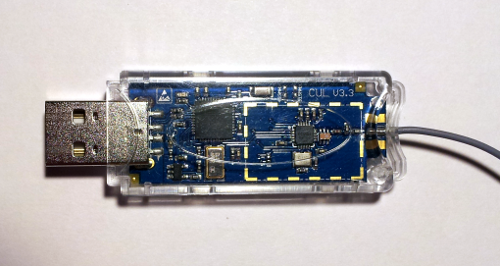
\includegraphics[width=\linewidth]{Cul}
			\begin{block}{Protokolle}
				\begin{itemize}
				\item 	Slow-RF: \linebreak
						\textbf{FS20}, \textbf{FHT}, EM, \linebreak
						S300, HMS, \ldots
				\item 	AskSin: \linebreak
						\textbf{HomeMatic}
				\end{itemize}
			\end{block}
		\end{column}
	\end{columns}
\end{frame}

\subsection{FS20}

\begin{frame}{FS20}

\begin{block}{Wirtschaftliche Lage}
\begin{itemize}
\item 	Verfügbarkeit: eine Vielzahl an Hardware
\item 	Preisniveau: moderat
\end{itemize}
\end{block}

\begin{block}{Eigenschaften}
\begin{itemize}
\item 	Nachrichtenaustausch: unverschlüsselt, keine Bestätigung
\item 	Pairing: simpel \eg{(Pairing-Modus aktivieren, Setzen von IDs via Kommandos)}
\item 	Unterscheidung zwischen Hauscode und Devicecode
\item 	Kommunikation: CUL \eg{(Firmware culfw)}
\end{itemize}
\end{block}
\end{frame}

\begin{frame}{FS20}{Stand}

\begin{block}<+->{Funksteckdose (FS20 ST-2)}
\begin{itemize}
\item 	Aktorknoten
\item 	reine FS20-Komponente
\item 	schaltbar \eg{(aus Python heraus)}
\end{itemize}
\end{block}

\begin{block}<+->{Funk-Tür-Fensterkontakt (FHT 80TF-2)}
\begin{itemize}
\item 	Sensorknoten
\item 	keine reine FS20-Komponente (FHT-Protokoll)
\item 	CUL unterstützt nicht nur FS20,
		sondern auch FHT und viele weitere Protokolle
\item 	Nachrichten werden empfangen und können ausgewertet werden
\end{itemize}
\end{block}
\uncover<3->{\alert{$\Rightarrow$ für den Prototypen ausreichend}}
\end{frame}

\subsection{HomeMatic}

\begin{frame}{HomeMatic}{Vergleich zu FS20}
		\centering
	\begin{tabular}{lcc}
	\toprule
	           & \textit{FS20} & \textit{HomeMatic} \tabularnewline
	\midrule
	Preisniveau & moderat & teuer \tabularnewline
	Gerätevielfalt & groß & klein \tabularnewline
	Frequenzband & \multicolumn{2}{c}{868 MHz} \tabularnewline
	Authentifizierung & keine & AES \tabularnewline
	Übertragung & unverschlüsselt & XOR-verschlüsselt  \tabularnewline
	Empfangsbestätigung & nein & ja  \tabularnewline
	\multirow{2}{*}{Sonstiges} & \multirow{2}{*}{Funktionsgruppen} & drahtgebundene \tabularnewline
	                           &                                   & Komponenten\tabularnewline
	\bottomrule
	\end{tabular}
\end{frame}

\begin{frame}{HomeMatic}{Stand / Vorgehen}
\begin{block}{Vorgehen}
\begin{itemize}
\item 	Analyse des Quellcodes von FHEM zum Verständnis des HomeMatic
		zugrunde liegenden Protokolls
\item 	Validierung des Protokolls durch Mitschnitte per CUL
\end{itemize}
\end{block}

\begin{block}{Stand}
\begin{itemize}
\item 	Funk-Zwischenstecker-Schaltaktor 1fach: Empfang und Auswertung des Paketes erfolgriech
\item 	Funk-Handsender 4 Tasten: Empfang und Auswertung des Paketes erfolgriech
\item 	Steuern eines Aktors ist noch offen
\end{itemize}
\end{block}
\end{frame}


\section{6LoWPAN}

\subsection{Routing (RPL)}

\begin{frame}{Routing in 6LoWPAN}{RPL}
		\begin{block}{}
			\begin{itemize}
			\item 	dynamisches Routing-Protokoll
					für energiearme und verlustbehaftete Netzwerke
			\item 	Route-Over-Protokoll
			\item 	Protokoll auf Basis eines Distanzvektor-Algorithmus:
					\begin{itemize}
					\item 	DODAG (Destination Oriented Directed Acyclic Graph)
					\item 	jeder Knoten besitzt einen Rang
					\item 	spezielle Nachrichten zum Austausch der
							Routing-Informationen \eg{(DIO, DIS, DAO)}
					\item 	Zielfunktion berechnet Rang
							und wählt bevorzugten Elternknoten
					\end{itemize}
			\item 	weitere Besonderheiten:
					\begin{itemize}
					\item 	Local und Global-Repair (z.B. bei Ausfall eines Knotens)
					\item 	Verwendung des Trickle Timer Algorithmus
					\end{itemize}
			\item 	Implementation in Contiki: ContikiRPL
					\begin{itemize}
					\item 	keine im Standard definierten Sicherheitsmechanismen implementiert
					\end{itemize}
			\end{itemize}
		\end{block}
\end{frame}

\begin{frame}{Routing in 6LoWPAN}{RPL}
	\begin{figure}
	\centering
	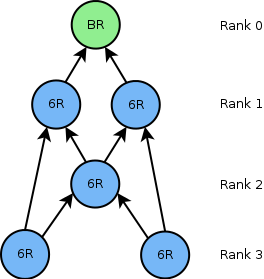
\includegraphics[width=0.5\linewidth]{Dodag}
	\linebreak
	\emph{Ein Beispielnetz}
	\end{figure}
\end{frame}
\subsection{Sensorknoten}

\begin{frame}{Sensorknoten letztes Semester}
	\begin{itemize}
	\item 	Sensor Terminal Board
			mit rcb128rfa1 Modul
	\item 	AVR ATmega128rfa1 Microcontroller
	\item 	Ansteuerung der Sensoren
			ohne Betriebssystem:
			\begin{itemize}
			\item 	Feuchtigkeitssensor
			\item 	Drucksensor
			\item 	Geschwindigkeitssensor
			\item 	Ansteuerung per I2C-Bus
			\end{itemize}
	\item 	Einarbeitung in Contiki:
			\begin{itemize}
			\item 	Wie können die Sensoren sinnvoll implementiert werden?
			\item 	Beachtung der Trennung von
					Core, CPU und Platform
			\item 	Nutzung bereits implementierter Schnittstellen
			\end{itemize}
	\end{itemize}
\end{frame}

\begin{frame}{Sensorknoten dieses Semester}
	\begin{itemize}
	\item 	deRFmega128-Board (Batteriebetrieb)
	\item 	AVR ATmega128rfa1 Microcontroller
	\item 	Verifizierung der I2C-Schnittstelle in Contiki durch neuen Sensor (Lichtsensor)
	\item 	Ansteuerung eines Aktors (Heizungsthermostat):
			\begin{itemize}
			\item 	zwei Boards, die per UART miteinander kommunizieren
			\item 	Software des Heizungsthermostat
					durch Bachelor-Projekt
					bereitgestellt
			\item 	das deRFmega128-Board stellt die Funk-Kommunikation bereit
			\end{itemize}
	\end{itemize}
\end{frame}


%\section[Fazit]{Schlussbemerkungen}
%-------------------------------------------------------------------------------
\begin{frame}{Schlussbemerkungen}
	\begin{itemize}
	\item	die \emph{Implementierung von} Contiki ist sehr verwoben
	\item	die \emph{Programmierung für} Contiki ist recht elegant
	\item	der Dokumentation fehlen Einführungen für das Systemverständnis
	\item 	die Netzwerk-Anbindung ist gut ausgebaut
	\item 	die Funktionalität im Net Stack sind klar getrennt
	\item 	die praktischen Einsatzmöglichkeiten des Dynamic Module Loading
			ist in Sensornetzen beschränkt
\end{itemize}
\end{frame}
%-------------------------------------------------------------------------------
\begin{frame}{Ausblick}
	\begin{itemize}
	\item 	Net Stack: Security--layer (ContikiSec)
	\item 	Sleep Modi einbauen
	\item 	Debug-System (bisher nur als Macro pro Datei)
	\item 	Echtzeit-Eigenschaften
	\end{itemize}
\end{frame}
%-------------------------------------------------------------------------------
\begin{frame}{Ausgewählte Quellen}
%	\begin{enumerate}
%	\item 	Farooq, O. M. \& Kunz, T. (2011):
%	\end{enumerate}
	\begin{thebibliography}{contiki12}
	\bibitem[contiki12]{OSforWSN:2011}
		Farooq, O. M. \& Kunz, T.:
		\emph{Operating Systems for Wireless Sensor Networks: A Survey},
		\url{www.mdpi.com/1424-8220/11/6/5900/pdf},
		2011
	\bibitem[contiki12]{DynReProgSensors:2008}
		Strübe, Jan Moritz:
		\emph{Dynamische Re-Programmierung von Sensorknoten zur Laufzeit},
		\url{strübe.de/wp-content/uploads/2008/08/da.pdf},
		Diplomarbeit,
		% Friedrich-Alexander-Universität Erlangen-Nurnberg,
		2008
	\bibitem[contiki12]{dunkels06:2006}
		Dunkels, Adam et al.:
		\emph{Run-Time Dynamic Linking for Reprogramming Wireless Sensor Networks}
		\url{dunkels.com/adam/dunkels06runtime.pdf},
		2006
	\end{thebibliography}
\end{frame}
%-----------------------------------------------------------------------------11

%-------------------------------------------------------------------------------

\end{document}
